\documentclass[12pt, letterpaper, twoside]{article}
\usepackage[T2A]{fontenc}
\usepackage{amsfonts}
\usepackage{amsmath}
\usepackage{mathabx}
\usepackage{graphicx}

\title{Лекции по математическому анализу 4 модуль.}
\author{Андрей Тищенко}
\date{2023/2024}

\newcommand{\tg}{\operatorname{tg}}
\newcommand{\Bold}[1]{$\textbf{#1}$}
\newcommand{\Underl}[1]{$\underline{\text{#1}}$}
\newcommand{\BU}[1]{$\underline{\textbf{#1}}$}
\newcommand{\DS}{\displaystyle}
\newcommand{\tr}{\operatorname{tr}}
\newcommand{\Rg}{\operatorname{Rg}}
\newcommand{\Hom}{\operatorname{Hom}}
\newcommand{\oo}{\infty}
\newcommand{\arctg}{\operatorname{arctg}}
\newcommand{\Abs}[1]{\left| #1 \right|}
\newcommand{\mb}[1]{\mathbb{#1}}

\begin{document}
    \maketitle
    \[\textbf{Лекция 12 апреля.}\]
    \[\text{Сходимость функциональных рядов}\]
    $f_n(x),\ n\in \mb{N},\ x\in E \subseteq \mb{R}$\\
    $f_n(x) \xrightarrow[n\rightarrow \oo]{} f(x)$
    \begin{enumerate}
        \item[Определение:] $f_n(x)\overset{E}{\rightrightarrows} f(x) \Leftrightarrow \DS \sup_{x\in E} |f_n(x) - f(x)| \xrightarrow[b\rightarrow \oo]{} 0$
        \item[Пример:] Закон больших чисел. $\eta_n(\omega) = \frac{\xi_1 (\omega) + \dots + \xi_n(\omega)}{n} \xrightarrow[n\rightarrow \oo]{} E\xi_1 = a$ почти наверное. $P \{\omega:\ \eta_n(\omega)\xrightarrow[n\rightarrow \oo]{} a\} = 1$
        \item[Вопрос:] можно ли переставлять операторы $\DS \lim_{n\rightarrow \oo},\ \lim_{x\rightarrow x_0},\ \frac{d}{dx},\ \int\, dx$?\\
        То есть $\DS \lim_{n\rightarrow \oo} \lim_{x\rightarrow x_0} f_n(x) \overset{?}{=} \lim_{x\rightarrow x_0} \lim_{n\rightarrow \oo} f_n(x)\\
        \lim_{n\rightarrow \oo} \frac{d}{dx} f_n(x) \overset{?}{=} \frac{d}{dx} \lim_{n \rightarrow \oo} f_n(x)\\
        \lim_{n\rightarrow \oo} \int f_n(x) dx \overset{?}{=} \int \left( \lim_{n\rightarrow \oo} f_n(x)\right)dx$\\
        Нет, нельзя.
        \item[Пример 1.] $f_n(x) = x^n,\ E = [0;\ 1],\ x_0 = 1\\
        \lim_{n\rightarrow \oo}\lim_{x\rightarrow 1^-} x^n = \lim_{n\rightarrow \oo} 1 = 1\\
        \lim_{x\rightarrow 1^-} \lim_{n\rightarrow \oo}x^n = \lim_{x\rightarrow 1^-} \begin{pmatrix}
            0, & x < 1\\
            1, & x = 1
        \end{pmatrix} = 0$
        \item[Теорема:] $f_n(x)$ непрерывна в точке $x_0 \in E$ и $f_n(x) \overset{E}{\rightrightarrows} f(x)$, то\\
        $f(x)$ непрерывна в точке $x_0$
        \item[Пример 2.] $f_n(x) = \frac{\sin nx}{n},\ x\in \mb{R},\ x_0 = 0\\
        f(x) \equiv 0\quad f'(0) = 0$\\
        $f'_n(x) = \frac{\cos nx}{n}\cdot n = \cos nx |_{n_0 = 0} \equiv 1 \xrightarrow[n\rightarrow \oo]{} 1$
        \item[Теорема:] $f_n(x)$ непрерывна и дифференцируема на $[a;\ b]$\\
        $\exists c\in [a;\ b]:\ f_n(c)$ сходится\\
        $f_n'(x) \overset{[a;\ b]}{\rightrightarrows}$, тогда\\
        $f_n(x) \overset{[a;\ b]}{\rightrightarrows}$ и $\DS\lim_{n\rightarrow \oo} \frac{d}{dx} f_n(x) = \frac{d}{dx} \lim_{n\rightarrow \oo} f_n(x)$
        \item[Пример 3.] $f_n(x) = $
        \scalebox{0.06}[0.04]{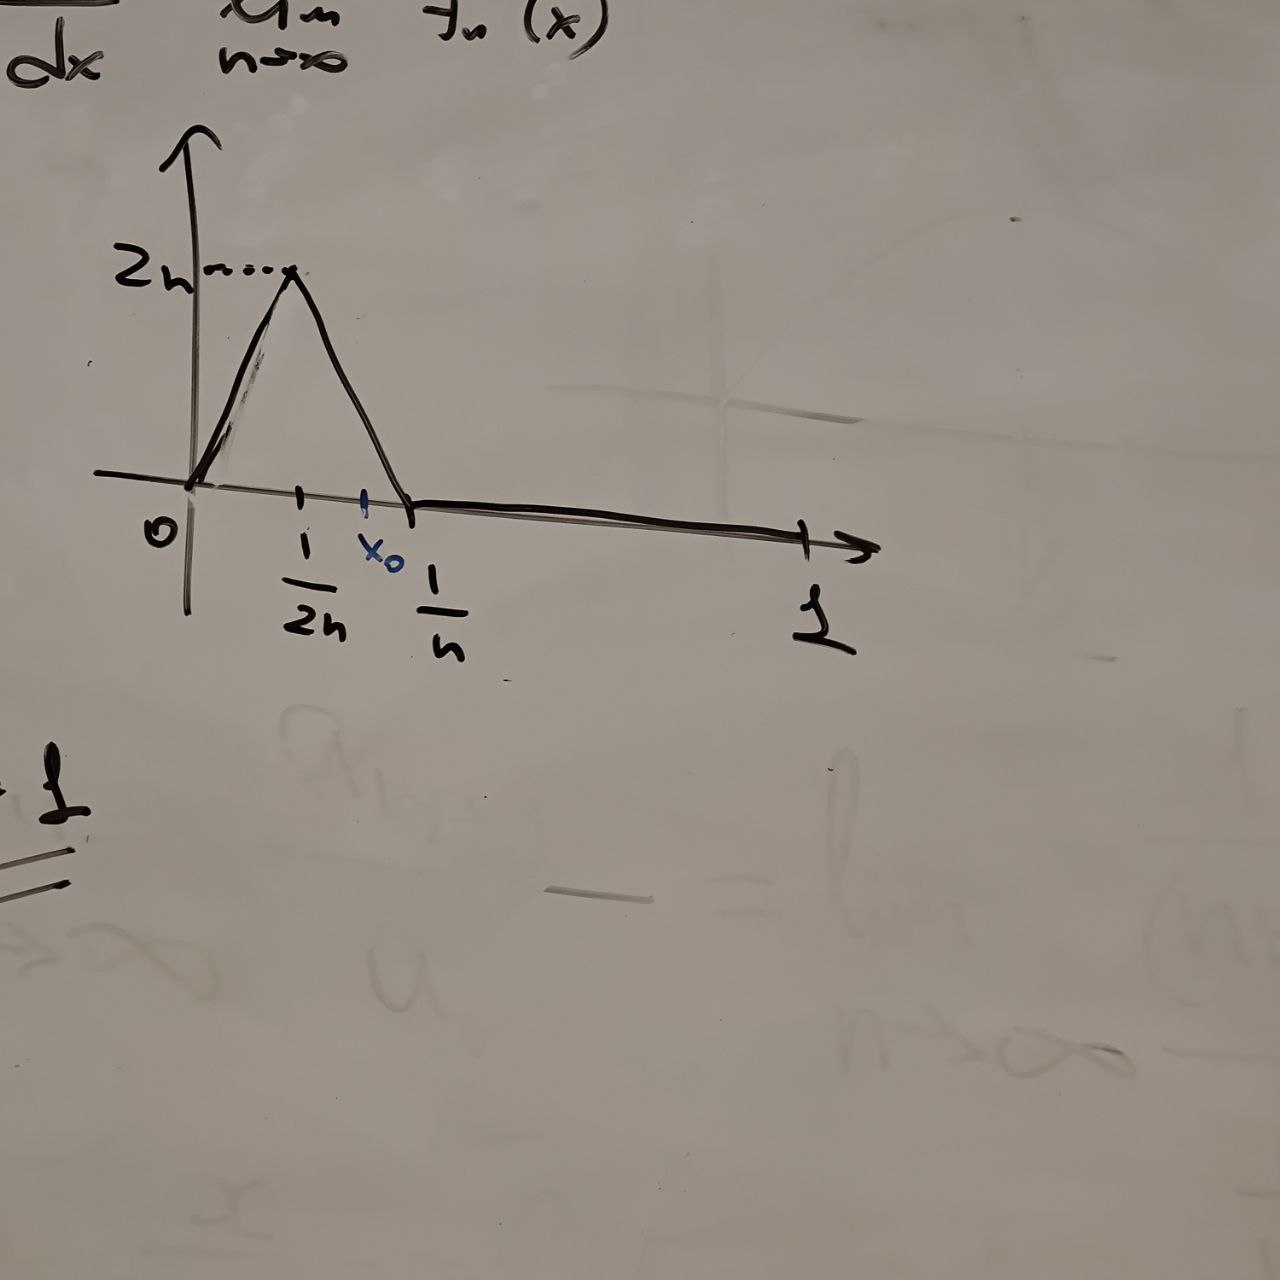
\includegraphics{../pictures/График матан1.jpg}} \\
        $\forall x\in [0;\ 1]\ f_n(x) \longrightarrow 0\\
        \DS \int_0^1 f_n(x)dx = 1,\ \lim_{n\rightarrow \oo} 1 = 1\\
        \int_0^1 f(x)dx = 0\neq 1$
        \item[Теорема:] $f_n(x) \overset{[a;\ b]}{\rightrightarrows} f(x)$, то\\
        $\forall c \DS \int_c^x f_n(t)dt \overset{[a;\ b]}{\underset{n\rightarrow \oo}{\rightrightarrows}} \int_c^x f(t)dt$\\
        \[\text{Сходимость функциональных рядов}\]
        $\DS \sum_{n = 1}^{\oo} u_n (x) = S(x),\ x\in E$\\
        Ряд сходится равномерно:\\
        $\DS\sup_{x\in E} \Abs{\sum_{k = 1}^{n}u_k(x) - S(x)} = \Abs{\sum_{k = n + 1}^{+\oo} u_k(x)} \xrightarrow[n\rightarrow \oo]{} 0$\\
        \item[Теорема:] (признак Вейерштрасса) если последовательность $u_n(x)$ мажорируется числовой последовательностью $a_n:\ \forall n\in \mb{N},\ \forall x\in E \Abs{u_n(x)}\leq a_n$. Тогда из сходимости $\DS \sum_{n =1}^{+\oo}u_n(x)$  следует сходимость $u_n(x)$ на $E$.\\
        \item[Пример:] $u_n(x) = $
        \scalebox{0.06}[0.04]{\includegraphics{../pictures/График матан2.jpg}}\\
        $\DS \sum_{k = 1}^{+\oo} u_n(x) = f(x)\\
        \sup_{x\in[0;\ 1]} \Abs{f(x) - \sum_{k = 1}^{n}u_k(x)}\leq \frac{1}{n} \xrightarrow[n\rightarrow \oo]{} 0$\\
        $\DS\sup_{x \in [0;\ 1]}\Abs{u_n(x)} = \frac{1}{n}\quad \sum_{n = 1}^{+\oo} \frac{1}{n}$ расходится.\\
        То есть мы имеем равномерную сходимость, но найти мажорирующую последовательность нельзя.\\
        Рассмотрим ряд $\DS \sum_{n = 1}^{+\oo} nx^{n - 1} = \sum_{n =1}^{+\oo} \overset{?}{=} \left( \sum_{n = 1}^{+\oo} x^n \right)' = \left( \frac{x}{1 - x} \right)'$
    \end{enumerate}
        \[\text{Степенные ряды}\]
    $\DS \sum_{n = 0}^{+\oo} C_n\cdot (x - a)^n\quad \sum_{n = 0}^{+\oo} C_nx^n$
    \begin{enumerate}
        \item[Лемма.] (Абеля)
        \begin{enumerate}
            \item[1.] $\sum_{n = 0}^{+\oo} C_nx^n$ сходится при $x = x_1$, то $\forall x_0: \Abs(x_0) < \Abs{x_1}$ ряд $\sum_{n = 0}^{+\oo} C_nx^n$ сходится
            \item[2.] $\sum_{n = 0}^{+\oo} C_nx^n$ расиходится при $x = x_2$, то $\forall x_0: \Abs(x_0) > \Abs{x_2}$ ряд $\sum_{n = 0}^{+\oo} C_nx^n$ расходится
        \end{enumerate}
        $C_n\cdot x_1^n \xrightarrow[n\rightarrow \oo]{} 0 \Rightarrow$ ограниченна $\Rightarrow \exists M\ \forall n\ \Abs{C_n\cdot x_1^n} < M$
        \item[Доказательство:] 1. $\DS \sum_{n = 0}^{+\oo} \Abs{C_n\cdot x_0^n} = \sum_{n = 0}^{+\oo} \Abs{C_n \cdot x_1^n \cdot \left( \frac{x_0}{x_1} \right)^n} \leq M\cdot \underset{\text{сходится}}{\underbrace{\sum_{n=  0}^{+\oo}q^n}}\Rightarrow$ сходится абсолютно\\
        2. Пусть сходится при $x = x_0\underset{\text{п. 1}}{\Rightarrow}$ сходится при $x = x_2\Rightarrow \bot$
        \item[Вывод:] Возможен один из трёх вариантов
        \begin{enumerate}
            \item $\sum_{n = 0}^{+\oo} C_nx^n$ сходится $\forall x\in \mb{R}$
            \item $\sum_{n = 0}^{+\oo} C_nx^n$ сходится только при $x = 0$
            \item $\exists R:\ \sum_{n = 0}^{+\oo} C_nx^n$ сходится на $(-R;\ R)$ (\Underl{множество сходимости}), а на $(-\oo,\ -R)\cup(R,\ +\oo)$ расходится. Это $R$ называется \Underl{радиусом сходимости} степенного ряда.
        \end{enumerate}
        \item[Теорема:] $\forall r:\ 0 < r < R$ ряд $\sum_{n = 0}^{+\oo} C_nx^n$ сходится равномерно на $[-r,\ r]$
        \item[Доказательство:] $\DS\sup_{[-r;\ r]} \Abs{\sum_{k = 0}^{n} C_k x^k - \sum_{k = 1}^{+\oo}C_kx^k} = \sup_{[-r;\ r]}\Abs{\sum_{k = n+1}^{+\oo} C_k x^k} \leq \sum_{k = n+1}^{+\oo}\Abs{C_k r^k}$, так как $r$ находится в множестве сходимости, значит $\underset{\text{числовой ряд}}{\underbrace{\sum_{k = n + 1}^{+\oo} C_k r^k}}$ сходится абсолютно.
        \item[Утверждение:] Если ряд $\DS\sum_{k =1}^{+\oo} a_k$ сходится и $\DS \sum_{k =1}^{+\oo} a_kx^k$ имеет радиус сходимости $R = 1$ и $\DS\lim_{x \rightarrow 1^-} f(x)$ существует, то 
        $\DS\sum_{k = 1}^{+\oo} a_k = \lim_{x \rightarrow 1^-} f(x)$.
        \item[Теорема:] 1. Если $\DS \lim_{n \rightarrow \oo} \Abs{\frac{C_n}{C_{n + 1}}} = A$, то $R = A$\\
        2. Если $\DS \lim_{n\rightarrow \oo} \sqrt[n]{\Abs{C_n}} = B$, то $R = \frac{1}{B}$
        \item[Доказательство:] 1. $\DS0 < A < +\oo\quad \sum_{n = 0}^{+\oo}C_n\cdot x^n\\
        \lim_{n \rightarrow \oo} \Abs{\frac{c_{n + 1}x^{n + 1}}{C_n x^n}} = \Abs{x}\cdot \lim_{n\rightarrow \oo}\Abs{\frac{C_{n + 1}}{C_n}} = \Abs{x}\frac{1}{A}\\
        \Abs{x} < A$ сходится по Даламберу\\
        $\DS \Abs{x} > A$ расходится по Даламберу, значит $R = A$\\
        2. $A = +\oo\quad \DS \lim_{n\rightarrow \oo} \Abs{\frac{C_{n + 1}x^{n + 1}}{C_n x^n}} = 0\Rightarrow \forall x$ по Даламберу сходится $R = +\oo$\\
        3. $A = 0\quad \DS \lim_{n \rightarrow \oo} \Abs{\frac{C_{n + 1}x^{n + 1}}{C_n x^n}} = +\oo\Rightarrow \forall x\neq 0$ расходится.
    \end{enumerate} 
    \[\textbf{Лекция 17 апреля}\] 
    \[\text{Степенные ряды}\]
    $\DS \sum_{n = 0}^{+\oo}c_n x^n$. Выполняется одно из трёх.\\
    \begin{enumerate}
        \item Сходится только при $x = 0$
        \item Сходится абсолютно $\forall x$
        \item Сходится абсолютно на $(-R;\ R)$, расходится на $(-\oo;\ -R)\cup (R;\ +\oo)$. R - радиус сходимости.
    \end{enumerate}
    \begin{enumerate}
        \item[Теорема:] $\forall r:\quad 0 < r < R_{\text{сх}}$ ряд сходится равномерно на $[-r;\ r]$
        \item[Теорема (Абеля):] Если рдя сходится при $x = R$ абсолютно, то на отрезке $[0;\ R]$ ряд сходится равномерно.
        \item[Теорема:] Если $\exists \DS \lim_{n\rightarrow \oo} \frac{\Abs{C_{n + 1}}}{\Abs{c_n}}\ (\exists \DS \lim_{n\rightarrow +\oo} \sqrt[n]{|c_n|}) = A \in \overline{\mb{R}}$, то\\
        $R_{\text{сх}} = \dfrac{1}{A}$
        \item[Доказательство:] $\DS \lim_{n\rightarrow \oo} \frac{\Abs{c_{n + 1} x^{n + 1}}}{\Abs{c_n x^n}} = \Abs{x} \lim_{n\rightarrow \oo} \Abs{\frac{c_{n  +1}}{c_n}} = \Abs{x}\cdot A\quad (*)$\\
        \begin{enumerate}
            \item[1 случай.] $A = 0$, $(*) < 1$, то есть сходимость при любом $x$,\\
            то есть $R_{\text{сх}} = +\oo$
            \item[2 случай.] $A = +\oo$ $(*) = +\oo > 1$, то есть расходимость при любом $x\neq 0$, то есть $R_{\text{сх}} = 0$
            \item[3 случай.] $A\in \mb{R}^+$ $|x| A < 1$ сходится, то есть $\Abs{x} < \dfrac{1}{A}$,\\
            $\Abs{x} A > 1$ расходится, то есть $\Abs{x} > \dfrac{1}{A}$\\
            То есть $R_{\text{сх}} = \dfrac{1}{A}$ 
        \end{enumerate}
        \item[Теорема:] (Формула Коши-Адамара)
        \[R_{\text{сх}} = \frac{1}{\overline{\lim\limits_{n\rightarrow \oo}}\sqrt[n]{\Abs{c_n}}}\]
        Доказывательства не будет.
    \end{enumerate}
    Вопрос:
    \[\sum_{n = 0}^{+\oo} f_n'(x) \overset{?}{=} \left( \sum_{n = 0}^{+\oo} f_n(x) \right)'\]
    Это не всегда верно, стоит запомнить данный факт.
    \begin{enumerate}
        \item $\DS \sum_{n = 0}^{+\oo} c_n x\quad R_1$
        \item $\DS \sum_{n = 0}^{+\oo} c_n n x^{n - 1} = \frac{1}{x} \sum_{n = 0}^{+\oo} c_n n x^n\quad R_2$
        \item $\DS \sum_{n = 0}^{+\oo} \frac{c_n}{n + 1} x^{n + 1} = x\sum_{n = 0}^{+\oo}\frac{c_n}{n + 1} x^n\quad R_3$
        \item[Теорема:] $R_1 = R_2 = R_3$
        \item[Доказательство:]
        \begin{enumerate}
            \item[1.] $R_2 \leq R_1 \leq R_3$ (очевидно из коэффициентов,\\
            так как $c_n n \geq c_n \geq \dfrac{c_n}{n + 1}$)\\
            Пусть $x_1$ - точка сходимости $2.$ то есть сходится $\DS \sum_{n = 0}^{+\oo}\Abs{c_n}\cdot \Abs{x_1}^n \cdot n$, тогда по признаку сравнения\\
            $\DS \sum_{n = 0}^{+\oo} \Abs{\frac{c_n}{n + 1}}\Abs{x_1}^n \leq \sum_{n = 0}^{+\oo} \Abs{c_n}\Abs{x_1}^n\leq \sum_{n = 0}^{+\oo}\Abs{c_n}\cdot \Abs{x_1}^n \cdot n$\\
            Все остальные ряды сойдутся.
            \item[2.] $R_3 \leq R_2$\\
            Если при $x_0$ сходится (абсолютно) $3.$, то при $x_0$ сходится $2.$\\
            $\DS \sum_{n = 0}^{+\oo} \Abs{\frac{c_n}{n + 1} x_1^n}$ - сходится $\Rightarrow\\
            \Rightarrow \exists M \forall n\ \Abs{\frac{c_n}{n + 1} x_1^n}\leq M\\
            \exists x_1:\quad \Abs{x_0} < \Abs{x_1} < R_3$\\
            $\DS\sum_{n = 0}^{+\oo} \Abs{c_n n x_0^n} = \sum_{n = 0}^{+\oo} \underset{\leq M}{\underbrace{\Abs{\frac{c_n}{n + 1}x_1^n}}}\cdot(n + 1)n\cdot \underset{q^n}{\Abs{\underbrace{\frac{x_0}{x_1}}}}^n \leq \\
            \leq M \sum_{n = 0}^{+\oo} n(n  + 1)q^n$ сходится по Даламберу ($0 < q < 1$)
        \end{enumerate} 
    \end{enumerate}
    \[\text{Выводы:}\]
    $\DS \sum_{n = 0}^{+\oo} c_n x^n = f(x),\quad D_f = (-R;\ R)$\\
    $\DS \sum_{n = 0}^{+\oo}c_n n x^{n + 1} = f'(x)\\
    \sum_{n = 0}^{+\oo} \frac{c_n}{n + 1} x^{n + 1} = \int_0^x f(t)\, dt$\\
    $f(x)$ - бесконечно число раз дифференцируем.\\
    $f^{(k)}(0) = c_k\cdot k!$
    \begin{enumerate}
        \item[Вывод:] Если $f(x)$ раскладывается в степенной ряд, то $c_k = \dfrac{f^{(k)}(0)}{k!}$
        \item[Пример:] $f(x) \begin{cases}
            e^{-\frac{1}{x^2}},\ x = 0\\
            0,\ x = 0
        \end{cases}\\
        f'(0) = \DS \lim_{x \rightarrow 0} \frac{e^{-\frac{1}{x^2}} - 0}{x - 0} = 0$
        \item[Утверждение:] $e^{-\frac{1}{x^2}} \dfrac{P_n(x)}{Q_m(x)}\xrightarrow[x\rightarrow 0]{} 0\\
        f^{(k)}(0) = \lim_{x\rightarrow  0} \dfrac{f^{(k + 1)}(x) - f^{(k - 1)}(0)}{x - 0} = 0\\
        \sum_{n = 0}^{+\oo} c_n x^n \equiv 0 \neq f(x)$, хотя функция бесконечное число раз дифференцируема. 
    \end{enumerate}
    \[\text{Ряды Тейлора}\]
    \begin{enumerate}
        \item[Определение:] Рядом Тейлора функции бесконечное число раз дифференцируемой в точке $x = a$ называется
    \end{enumerate}
    \[\sum_{n = 0}^{+\oo} \frac{f^{(n)}(a)}{n!}(x - a)^n\quad (*)\]
    \begin{enumerate}
        \item[Теорема:] (Достаточное условие) Если $f^{(k)}(x)$ ограничена в совокупности на интервале $(a - R;\ a + R)$, то $(*)$ верно на $(a - R;\ a + R)$
        \item[Доказательство:] ограничена в совокупности означает: 
        \[\exists M\ \forall k\ \forall x\in U_R(a):\ \Abs{f^{(k)}} \leq M\]
        $\DS \Bigg|{\underset{T_k(x)}{\underbrace{\sum_{n = 0}^{k} \frac{f^{(n)}(a)}{n!}(x - a)^n}} - f(x) }\Bigg| = \Abs{ \frac{f^{(k + 1)}(\xi)\cdot (x - n)^{k + 1}}{(k + 1)!} } \leq$\\
        $\leq \frac{M\cdot R^{k + 1}}{(k + 1)!}\xrightarrow[k\rightarrow +\oo]{}0$ 
    \end{enumerate}
    \begin{enumerate}
        \item[1.] $y = e^x\\
        \Abs{f^{(k)}(x)} = \Abs{ e^x } \leq e^{R}\\
        \forall x\ e^x =\DS \sum_{n = 0}^{+\oo} \frac{x^n}{n!}$
        \item[2.] $y = \sin x\\
        \Abs{ f^{(k)}(x) } \leq 1\\
        \forall x \sin x = \DS \sum_{n = 0}^{+\oo} \frac{ (-1)^n }{ (2n + 1)! } x^{2n + 1}$
        \item[3.] $y = \cos x\\
        \DS\forall x\ \sum_{n = 0}^{+\oo} \frac{ (-1)^n }{(2n)!} x^{2n}$
    \end{enumerate}
    В комплексных числах $\DS f(z) = \sum_{n = 0}^{+\oo} c_n z^n$ аналитические функции (для них радиус сходимости выглядит так $|z| < R$)
    \begin{enumerate}
        \item[4.] $y = \ln(1 + x), a = 0\\
        y' = \dfrac{1}{1 + x} = \DS \sum_{n = 0}^{+\oo} (-1)^n x^n,\ |x| < 1\\
        \int_0^x \frac{1}{1 + t}\, dt = \sum_{n = 0}^{+\oo} \int_0^x (-1)^n t^n\, dt = \sum_{n = 0}^{+\oo} \frac{(-1)^n}{n + 1}x^{n + 1}$\\
        Но $\ln(1 + x): x \in (-1;\ +\oo)$, а $\DS \sum_{n = 0}^{+\oo} \frac{(-1)^n}{n + 1}x^{n + 1}: x \in (-1;\ 1]$
        \item[5.] $(1 + x)^{\alpha} = \DS \sum_{n  = 0}^{+\oo} c_n^{\alpha} x^n \alpha (\alpha - 1)\dots(\alpha -n + 1)$
    \end{enumerate}
    \newpage
    \[\textbf{Лекция 19 апреля}\]
    \[\textbf{Многомерный анализ}\]
    
    $f: \mathbb{R}^n\to \mathbb{R};\quad f(\vec{x}); \quad \vec{x} = (x_1, \dots, x_n)$\\
    \begin{enumerate}
        \item[{\textbf{Определение:}}] \textbf{(Коши)}
    \end{enumerate}
$\lim\limits_{\vec{x}\to \vec{x}_0} f(\vec{x}) = A\Leftrightarrow \forall \varepsilon > 0 \exists \delta = \delta(\varepsilon)>0 \forall \vec{x}: \vec{x} \in U\circ_\delta (\vec{x_0})$
$$|f(\vec{x} - A)| < \varepsilon$$
\begin{enumerate}
    \item [\textbf{Определение:}] 
\end{enumerate}
$$\vec{x} \in U\circ_\delta (\vec{x}_0) \Leftrightarrow 0 < \rho(\vec{x}, \vec{x}_0) < \delta$$
\begin{enumerate}
    \item[\textbf{Определение:}] 
\end{enumerate}
    метрическим пространством называется $(M, \rho)$: $\forall x, y$
\begin{enumerate}
    \item[1] $\rho (x, y) = \rho (y ,x) \geq 0$
    \item[2] $\rho (x, y) = 0 \Leftrightarrow x = y$
    \item[3] $\forall x, y, z\quad \rho (x, z) \leq \rho (x, y) + \rho (z, y)$
\end{enumerate}
Классическая метрика на $\mathbb{R}_n$
$$\rho(\vec{x}, \vec{y}) = \sqrt{(x_1 - y_1)^2 + \dots + (x_n - y_n)^2}$$
\begin{enumerate}
    \item[\textbf{Определение:}] \textbf{(Гейне)}
\end{enumerate}
$\lim\limits_{\vec{x}\to \vec{x}_0} f(\vec{x}) = A\Leftrightarrow\forall \vec{x_k}:\ \vec{x_k}\underset{k\to\infty}{\longrightarrow} \vec{x_0}\ \vec{x_k} \neq \vec{x_0} \Rightarrow f(\vec{x_k})\underset{k\to\infty}{\longrightarrow}A$

\textbf{Определение 1:}
$\vec{x}_k\underset{k\to\infty}{\longrightarrow} \vec{x_0} \Leftrightarrow \forall i: 1 \leq i \leq n\quad x_{i, k} \underset{k\to\infty}{\longrightarrow} x_{i, 0}$

\textbf{Определение 2:}
$\vec{x}_k\underset{k\to\infty}{\longrightarrow} \vec{x_0} \Leftrightarrow \rho({\vec{x_k}, \vec{x_0}}) \underset{k\to\infty}{\longrightarrow} 0$
\begin{enumerate}
    \item[\textbf{Теорема:}] \textbf{Определение 1 $\Leftrightarrow$ Определение 2}
\end{enumerate}
\subsection*{$1 \Rightarrow 2$}
$$\sqrt{\sum_{i = 1}^{n} (x_{i, k} - x_{i, 0})^2}\underset{k\to\infty}{\longrightarrow} 0\quad \text{по арифметике пределов последовательнотей}$$
\subsection*{$1 \Leftarrow 2$}
$$|x_{i, k} - x_{i, 0}| \leq \rho(\vec{x_k}, \vec{x_0})\underset{k\to\infty}{\longrightarrow} 0$$

\begin{enumerate}
    \item[\textbf{Замечание 1:}]
\end{enumerate}
Наследуется вся арифметика пределов
\begin{enumerate}
    \item[\textbf{Замечание 2:}]
\end{enumerate}
Тяжело доказывается сходимость\\

Там далее примеры были, но нам пофигу, сам там напишешь. ОК, спасибо, Вова.
\begin{enumerate}
    \item[\textbf{Определение:}]
\end{enumerate}
$f(\vec{x})$ называется непрерывной в точке $\vec{x_0} \Leftrightarrow\lim\limits_{\vec{x}\to \vec{x_0}}f(\vec{x}) = f(\vec{x_0})$
\begin{enumerate}
    \item[\textbf{Теорема:}]
\end{enumerate}
Функция непрерывна на компакте
\begin{enumerate}
    \item [1] ограничена на нём
    \item [2] достигаются наибольшее и наименьшее значение
    \item [3] принимает все промежуточные значения
\end{enumerate}
\begin{enumerate}
    \item[\textbf{Определение:}]
\end{enumerate}
Множество называется компактом, если для любого покрытия открытыми множествами существует конечное подпокрытие.
$$K \subset \bigcup_{\alpha}A_\alpha\ \exists \text{ конечный набор } A_{\alpha_1}, \dots, A_{\alpha_m}:$$
$$K \subset \bigcup_{\alpha}^mA_{\alpha_i}$$\newpage
\begin{enumerate}
    \item[\textbf{Определение:}]
\end{enumerate}
В $\mathbb{R}^n$ компактами являются ограниченные и замкнутые множества.

$$U_\delta(\vec{x_0}) = \{ \vec{x}:\ \rho (\vec{x}, \vec{x_0}) < \delta \}$$
\begin{enumerate}
    \item[\textbf{Определение:}]
\end{enumerate}
множество $A$ называется открытым $\Leftrightarrow \forall \vec{x} \in A\ \exists \delta > 0:
\ U_\delta(\vec{x})\subset A$
\begin{enumerate}
    \item[\textbf{Пример:}]
\end{enumerate}
$A\subseteq \mathbb{R}\quad A$ открыты $\Leftrightarrow A = \bigsqcup\limits_{k = 1}^{(n)+\infty} (a_k, b_k),\quad a_i, b_i\in \overline{\mathbb{R}}$\\
\begin{enumerate}
    \item[\textbf{Определение:}]
\end{enumerate}
множество $B$ называется замкнутым, если $\overline{B}$ - открыто\\
\begin{enumerate}
    \item[\textbf{Теорема:}]
\end{enumerate}
$A_i$ - открыто, $B_i$ - замкнуто
\begin{enumerate}
    \item [1] $\bigcup\limits_i A_i$ - открыто
    \item [2] $\bigcap\limits_i A_i$ - открыто
    \item [3] $\bigcap\limits_i B_i$ - замкнуто
    \item [4] $\bigcup\limits_i B_i$ - замкнуто
\end{enumerate}
\begin{enumerate}
    \item[\textbf{Пример (2):}]
\end{enumerate}
$$\bigcap_{n = 1}^{+\infty}\left( 0 - \dfrac{1}{2^n}; 1 + \dfrac{1}{2^n} \right) = [0 ,1]$$
\newpage\begin{enumerate}
    \item[\textbf{Пример (4):}]
\end{enumerate}
$$\bigcup_{n = 1}^{+\infty}\left[\dfrac{1}{n}; 1 - \dfrac{1}{n}\right] = (0, 1)$$
\begin{enumerate}
    \item[\textbf{Доказательство:}]
\end{enumerate}
\begin{enumerate}
    \item [1] $\bigcup\limits_i A_i = A$   $$\vec{x}\in A\Rightarrow \exists i\ \vec{x} \in A_i \Rightarrow \exists \delta: U_\delta(\vec{x})\subset A_i\Rightarrow U_\delta(\vec{y_0})\subset A$$
    \item [3] $\bigcap\limits_i B_i = \overline{\bigcup\limits_i \overline{B_i}}$ - замкнуто
    \item [4] $\bigcup\limits_{i = 1}^{k} B_i$\\
    Возьмем $\forall \vec{x_n}\in B$ и $\vec{x_n} \underset{n\in\infty}{\longrightarrow} \vec{x_0}\quad \exists i$ и  $\exists n_k$
    $$\forall k\ \vec{x_{n_k}}\in B_i\wedge \vec{x_{n_k}} \underset{n\in\infty}{\longrightarrow} \vec{x_0}\Rightarrow \vec{x_0}\in B_i \Rightarrow \vec{x_0}\in B$$
\end{enumerate}
\begin{enumerate}
    \item[\textbf{Теорема:}]
\end{enumerate}
множество $B$ замкнуто $\Leftrightarrow$ 
$$\forall \vec{x_k} \in B:\ \vec{x_k} \underset{k\to\infty}{\longrightarrow}\vec{x_0}
\Rightarrow \vec{x_0} \in B$$
\begin{enumerate}
    \item[\textbf{Доказательство:}]
\end{enumerate}
\subsection*{$"\Rightarrow"$}
Предположим противное, то есть $B$ замкнуто, но $\exists \vec{x_k} \in B:\ \vec{x_k} \underset{k\to\infty}{\longrightarrow}\vec{x_0}
\wedge \vec{x_0} \notin B$, то есть $\vec{x_0}\in \overline{B} - \text{открытое}$\\
$$\exists \delta:\ U_\delta(\vec{x_0})\subset \overline{B}$$
так как $\vec{x_k} \underset{k\to\infty}{\longrightarrow}\vec{x_0}\Rightarrow \exists N = N(\delta):\ \forall k > N\ \vec{x_k}\in U_\delta(\vec{x_0})\subset \overline{B}$ - противоречие.
\subsection*{$"\Leftarrow"$}
$B$ - замкнуто $\Leftrightarrow\ \overline{B}$ - открыто. \quad $\vec{y_0}\in \overline{B}\ \exists \delta:\ U_\delta(\vec{y_0})\subset \overline{B}$\\
Предположим противное, то есть $\delta_n = \dfrac{1}{n}$, то $\exists y_n\in U_\delta(\vec{y_0}) \wedge \vec{y_n} \notin \overline{B}\ (\text{то есть } \vec{y_n}\in B)$
Получаем $\vec{y_n} \underset{n\in\infty}{\longrightarrow} \vec{y_0}\Rightarrow \vec{y_0}\in B$ - противоречие\newpage
    \[\textbf{Лекция 26 апреля}\]
    \[\text{Дифференцируемость функции многих переменных.}\]
    \begin{enumerate}
        \item[\textbf{n = 1}]
    \end{enumerate}
    \[f'(x_0) = \underset{\text{производная}}{\lim_{x\to x_0} \frac{f(x) - f(x_0)}{x - x_0}}\Leftrightarrow f(x) = \underset{\text{дифференциал}}{f(x_0) + A(x - x_0) + \overline{o}\big((x - x_0)\big)}\]
    \begin{enumerate}
        \item[\textbf{n > 1}]
    \end{enumerate}
    Частные производные:
    \[\frac{\vartheta f(x;\ y)}{\vartheta x} := \lim_{\Delta x\to 0} \frac{f(x + \Delta x;\ y) - f(x;\ y)}{\Delta x}\]
    \begin{enumerate}
        \item[\textbf{Пример:}]
    \end{enumerate}
    \[f(x,\ y) = \begin{cases}
        \frac{xy}{x^2 + y^2},\ x^2 + y^2 \neq 0\\
        0,\ \text{иначе}
    \end{cases}\]
    \[\left. \frac{\vartheta f(x,\ y)}{\vartheta x}\right|_{\underset{y = 0}{x = 0}} = (0)_x' = 0\]
    \[\left. \frac{\vartheta f(x,\ y)}{\vartheta x} \right|_{\underset{y = 0}{x = 0}} = 0\]
    $\varDelta f =$ линейная функция от $(\Delta x_1,\dots,\ \Delta x_n) + \overline{o}\big(\rho(\vec{x},\ \vec{x}_0)\big)$
    \begin{enumerate}
        \item[\textbf{Определение:}] $(n = 2)$
    \end{enumerate}
    Функции $f(x)$ называется дифференцируемой в точке $(x_0,\ y_0)$, если
    \[f(x,\ y) = f(x_0,\ y_0) + A(x - x_0) + B(y - y_0) + \overline{o}\left( \sqrt{(x - x_0)^2 + (y - y_0)^2} \right)\]\newpage
    \begin{enumerate}
        \item[\textbf{Теорема:}]
    \end{enumerate}
    Если $f(x,\ y)$ дифференцируема в точке $(x_0,\ y_0)$, то 
    \[\exists \left.\frac{\vartheta f(x,\ y)}{\vartheta y}\right|_{\underset{y = y_0}{x = x_0}}\]
    и $A = \dfrac{\vartheta f}{\vartheta x},\ B = \dfrac{\vartheta f}{\vartheta y}\quad (x_0,\ y_0)$ и $f(x,\ y)$ непрерывна в $(x_0,\ y_0)$, $\vec{x} = \begin{pmatrix}
        x\\
        y
    \end{pmatrix},\ \vec{x}_0 = \begin{pmatrix}
        x_0\\
        y_0
    \end{pmatrix}$
    \begin{enumerate}
        \item[\textbf{Доказательство:}]
    \end{enumerate}
    $f(\vec{x}) - f(\vec{x}_0) = A\underset{\rightarrow 0}{(x - x_0)} + B\underset{\to 0}{(y - y_0)} + \overline{o}\big(\underset{\to 0}{\rho(\vec{x},\ \vec{x}_0)}\big)\\
    f(x,\ y_0) = f(x_0,\ y_0) + A(x - x_0) + \overline{o}\big(|x - x_0|\big)$\\
    Из курса матанализа можно сказать $\exists \dfrac{\vartheta f}{\vartheta x}$ и $A$ равен ему. 
    \begin{enumerate}
        \item[\textbf{Теорема:}] (достаточное условие дифференцируемости функции)
    \end{enumerate}
    Если $\dfrac{\vartheta f}{\vartheta x},\ \dfrac{\vartheta f}{\vartheta y}$ существует в некоторой окрестности точки $(x_0,\ y_0)$ и непрерывна в точке $(x_0,\ y_0)$, то функция дифференцируема в точке $(x_0,\ y_0)$
    \begin{enumerate}
        \item[\textbf{Пример:}]
    \end{enumerate}
    \[f(x,\ y) = \begin{cases}
        \frac{xy}{x^2 + y^2},\ x^2 + y^2 \neq 0\\
        0,\ \text{иначе}
    \end{cases}\]
    $\dfrac{\vartheta f}{\vartheta x} = \dfrac{y(x^2 + y^2) - 2x(xy)}{(x^2 + y^2)^2} = \dfrac{y^3 - x^2y}{(x^2 + y^2)^2}\Rightarrow \neg \exists \lim\\
    \dfrac{\vartheta f}{\vartheta y} = \dfrac{x^3 - xy^2}{(x^2 + y^2)^2}\Rightarrow \neg \exists \lim$
    \begin{enumerate}
        \item[\textbf{Доказательство:}]
    \end{enumerate}
    $f(x_0 + \Delta x;\ y_0 + \Delta y) - f(x_0;\ y_0) = \underset{=\frac{\vartheta f}{\vartheta y}(x_0 + \Delta x;\ y_0 + \Delta y \Theta 1)\Delta y}{f(x_0 + \Delta x;\ y_0 + \Delta y) - f(x_0 + \Delta x;\ y_0)} +\\
    + \underset{=\frac{\vartheta f}{\vartheta x}(x_0 + \Theta 2 \Delta x; y_0\ )\Delta x}{f(x_0 + \Delta x;\ y_0) - f(x_0;\ y_0)}=\dfrac{\vartheta f}{\vartheta y}(x_0;\ y_0)\Delta y + \dfrac{\vartheta f}{\vartheta x}(x_0;\ y_0)\Delta x + \overline{o}(1) +\\
    + \Delta y \overline{o}(1) + \Delta x\overline{o}(1)$, здесь $0 < \Theta_1,\ \Theta_2 < 1$\\
    Докажем, что $\Delta x\cdot \overline{o}(1) = \overline{o}(\sqrt{\Delta x^2 + \Delta y^2})\Rightarrow\\
    \Rightarrow \dfrac{\Delta x}{\sqrt{\Delta x^2 + \Delta y^2}}\cdot \overline{o}(1)\xrightarrow[\sqrt{\Delta x^2 + \Delta y^2}]{} 0$\\
    Итак, мы нашли нужные коэффициенты и представили функцию как сумму с нужным порядком малости.
    \begin{enumerate}
        \item[\textbf{1.}] Производная сложной функции.
    \end{enumerate}
    \begin{align*}
        f(\vec{x}) \oplus \vec{x}(t) =& \big(x_1(t),\dots,\ x_n(t)\big)\\
        f\big(\vec{x}(t)\big) =& g(x)
    \end{align*}
    \begin{enumerate}
        \item[\textbf{Теорема:}] $(n = 2)$
    \end{enumerate}
    Если $f(x;\ y)$ дифференцируема в точке $(x_0,\ y_0)$, $\begin{matrix}
        x = x(t)\\
        y = y(t)
    \end{matrix}$ дифференцируема в точке $t_0$: $\begin{matrix}
        x(t_0) = x_0\\
        y(t_0) = y_0
    \end{matrix}$, то
    \[g'(t) = \dfrac{dg(t)}{dt} = \frac{\vartheta t}{\vartheta x} (x_0,\ y_0)\cdot \left.\dfrac{d x(t)}{dt}\right|_{t = t_0} + \frac{\vartheta t}{\vartheta y} (x_0;\ y_0)\cdot \left.\frac{d y(t)}{dt}\right|_{t = t_0} = f'_x x'_t + f'_y y'_t\]
    \begin{enumerate}
        \item[\textbf{Доказательство:}]
    \end{enumerate}
    $f(x,\ y) = f(x_0,\ y_0) + f'_x(x - x_0) + f'_y(y - y_0) + \overline{o}\left(\sqrt{\Delta x^2 + \Delta y^2}\right)
    \dfrac{g(t) - g(t_0)}{t - t_0}= \dfrac{f\big( x(t),\ y(t)\big) - f(x_0,\ y_0)}{t - t_0} = f'_x\underset{x'_t}{\underbrace{\dfrac{x(t) - x(t_0)}{t - t_0}}} + f'(y)\underset{y'_t}{\underbrace{\dfrac{y(t) - y(t_0)}{t - t_0}}} + \sqrt{\left( \frac{\Delta x}{\Delta t}\right)^2 + \left( \frac{\Delta y}{\Delta t}\right)^2} +\\
    +\overline{o}(1)$\\
    $\sqrt{\left( \frac{\Delta x}{\Delta t}\right)^2 + \left( \frac{\Delta y}{\Delta t}\right)^2} \xrightarrow[t \to t_0]{} \sqrt{\left( x'_t\right)^2 + \left( y'_t\right)^2}$
    \begin{enumerate}
        \item[\textbf{2.}] Производная по направлению.
    \end{enumerate}
    $\vec{e}\ \Abs{\vec{e}} = 1\\
    \vec{e} = \{e_1,\ e_2,\dots,\ e_n\}\\
    \dfrac{\vartheta f}{\vartheta \vec{e}} = \DS \lim_{t\to 0} \frac{f(x_1 + e_1 t,\ x_2 + e_2 t,\dots,\ x_n + e_n t) - f(x_1,\dots,\ x_n)}{t}$\\
    $\DS \dfrac{dg(t)}{dt} = \frac{\vartheta t}{\vartheta x} (x_0,\ y_0)\cdot \left.\dfrac{d x(t)}{dt}\right|_{t = t_0} + \frac{\vartheta t}{\vartheta y} (x_0;\ y_0)\cdot \left.\frac{d y(t)}{dt}\right|_{t = t_0} = \sum_{i = 1}^{n} \frac{\vartheta f}{\vartheta x_i}\cdot e_i =\\
    =(\bigtriangledown \vec{f},\ \vec{e})\in \mathbb{R}$\\
    При этом $\bigtriangledown \vec{f}$ называется \Underl{градиентом} функции $f$\\
    Получается, что наибольшее значение производной по направлению получается, когда вектор $\vec{e}$ сонаправлен с вектором $\bigtriangledown \vec{f}$
    \[\textbf{Лекция 10 мая.}\]
    $f:\mb{R}^n\to \mb{R}$
    \begin{enumerate}
        \item[1.] Предел + непрерывность + свойства непрерывности.
        \item[2.] Дифференцируемость $\to$ не понятно.\\
        $f(\vec{x}) = f(\vec{x}_0) + \DS\sum_{i = 1}^{n} A_i(x^i - x^i_0) + \overline{o}\big(\rho(\vec{x};\ \vec{x}_0)\big)$
    \end{enumerate}
    Производная по направлению:
    \[\frac{\vartheta f}{\vartheta \vec{l}} = \lim_{t\to 0} \frac{f(\vec{x}_0 + t\vec{l}) + f(\vec{x}_0)}{t},\ \Abs{\vec{l}} = 1\]
    $\dfrac{\vartheta f}{\vartheta \vec{l}}\to max$, если $\vec{l}$ - градиент. \\
    $\DS\frac{\vartheta f}{\vartheta\vec{l}} = \frac{dg(t)}{dt} = \frac{d}{dt}\left( \vec{f} (\vec{x}_0 + t\vec{l})\right) = \sum_{i = 1}^{n} \frac{\vartheta f}{\vartheta x_i}\cdot \frac{d(x_i)}{dt}$, где $x_i = x_i^0 + tl_i$, тогда это равно:
    \[\sum_{i = 1}^{n} f_{x_i}'l_i = \left< grad\ \vec{f},\ \vec{l} \right> = \operatorname{proj}_{\vec{e}}\ grad\ \vec{f}\]
    proj - проекция.\\
    Итак, $\dfrac{\vartheta f}{\vartheta \vec{l}}\to max \Leftrightarrow \vec{e}\upuparrows grad\ \vec{f},\quad \max \dfrac{\vartheta f}{\vartheta \vec{e}} = \Abs{grad\ \vec{f}}$
    \begin{enumerate}
        \item[\textbf{Вывод:}]
    \end{enumerate}
    \begin{enumerate}
        \item[\textbf{Определение:}]
    \end{enumerate}
    Линией уровня функции $y = f(\vec{x})$ называется множество точек $\in \mb{R}^n$ таких, что
    \[f(\vec{x}) = c,\ \forall c\in \mb{R}\]
    \begin{enumerate}
        \item[\textbf{Утверждение:}]
    \end{enumerate}
    $grad\ \vec{f}\big|_{\vec{x}_0}$ перпендикулярен линии уровня $f(\vec{x}) = \underset{c}{\underbrace{f(\vec{x}_0)}}$\\
    $f\big(\vec{x}(t)\big) = c\ \forall t$\\
    Запараметризуем линию уровня:\\
    \[\frac{d}{dt} f\big(\vec{x}(t)\big) = 0\]
    \[\sum_{i = 1}^{n} \frac{\vartheta f}{\vartheta x_i}\cdot \frac{dx_i}{dt} = 0\Rightarrow (grad\ \vec{f};\ \vec{v}) = 0\Rightarrow \text{ Перпендикулярно.}\]
    \[\text{Неявно заданные функции}\]
    $y = f(x)\\
    F(x,\ y) = 0$\\
    Хотим найти $y = f(x):\ \forall x\  F(x,\ f(x)) = 0$
    \begin{enumerate}
        \item[\text{Пример:}]
    \end{enumerate}
    $y = \pm\sqrt{1 - x^2}\Rightarrow f(x) = \begin{cases}
        \sqrt{1 - x^2},\ -\frac{1}{2} \leq x \leq \frac{1}{2}\\
        -\sqrt{1 - x^2},\ \frac{1}{2 < |x| \leq 1}
    \end{cases}$
    \begin{enumerate}
        \item[\text{Определение:}]
    \end{enumerate}
    Функция $F(x,\ y) = 0$, заданная на $A \subseteq \mb{R}^2$\\
    $\exists y = f(x)\quad D_f = B\subseteq \operatorname{proj}_x A\\
    \forall x\in B:\quad F\big(x,\ f(x)\big) = 0$, то\\
    $y = f(x)$ называется неявной функцией, определяемой $F(x,\ y) = 0$
    \begin{enumerate}
        \item[Лемма:]
    \end{enumerate}
    $F(x,\ y)$ непрерывна на $U_{\xi}(x_0) \times U_{\eta}(y_0)$ и $F(x_0,\ y_0) = 0$
    $\forall x\in U_{\xi}(x_0)\quad F(x,\ y)$ строго монотонна по $y$, тогда:
    \[\exists \delta,\ \varepsilon\ \forall x\in U_{\delta}(x_0)\ \exists! y\in U_{\epsilon}(y_0):\ F(x,\ y) = 0\]
    Обозначим $y = f(x) \leftarrow$ непрерывна в точке $x_0$\newpage
    \begin{enumerate}
        \item[\text{Доказательство:}]
    \end{enumerate}
    Знаем $F(x_0,\ y_0) = 0$. Пусть она возрастает.\\
    Возьмём $\varepsilon < \eta\\
    F(x_0,\ y_0 + \varepsilon) > 0\\
    F(x_0,\ y_0 - \varepsilon) < 0\\
    \exists \delta$ в $\delta$-окрестности точки $(x_0,\ y_0 + \varepsilon)\ F(x,\ y) > 0$,\\
    в $\delta$-окрестности $(x_0,\ y_0 - \varepsilon)\ F(x,\ y) < 0$\\
    Возьмём $x \in U_{\delta}(x_0):\ F(x,\ y_0 - \varepsilon) < 0 \wedge F(x,\ y_0 + \varepsilon) > 0\Rightarrow\\
    \Rightarrow \exists! y \in (y_0 - \varepsilon,\ y_0 + \varepsilon):\ F(x,\ y) = 0$. Существование из непрерывности, единственность из строгой монотонности.\\
    Из доказательства для любого $\varepsilon$ найдётся $\delta$, что для всех $x$ из окрестности найдётся единственное $y$ из окрестности, то есть $y=f(x)$ монотонна.
    \begin{enumerate}
        \item[Теорема:] (о неявной функции)
    \end{enumerate} 
    $F(x,\ y)$ непрерывна в некоторой окрестности $(x_0,\ y_0)$ и $\exists F'_y(x,\ y)$ непрерывна в точке $(x_0,\ y_0)$, $F(x_0,\ y_0) = 0\quad F'_y(x_0,\ y_0) \neq 0$, то
    \[\exists \delta\ \exists \varepsilon\ \forall x\in U_{\delta}(x_0)\ \exists! y\in U_{\varepsilon}(y_0):\ F(x,\ y) \neq 0\]
    $y = f(x)$ непрерывна в точке $x_0$
    \begin{enumerate}
        \item[Бонус:]
    \end{enumerate}
    Если $\exists F'_x(x,\ y)$ в окрестности т. $(x_0,\ y_0)$ и есть непрерывность в точке $(x_0,\ y_0)$, то
    \[\exists f'(x_0) = -\dfrac{F'_x(x_0,\ y_0)}{F'_y (x_0,\ y_0)}\]
    \begin{enumerate}
        \item[Пример:]
    \end{enumerate}
    $\cos xy + x = 0\\
    y = f(x)\quad x\cos x f(x) + x = 0\\
    F\big(x,\ f(x)\big) = 0\\
    \frac{\vartheta F}{\vartheta x} + \frac{\vartheta F}{\vartheta y}\frac{f(x)}{dx} = 0\\
    \sin x f(x) (f(x) + xf'(x)) + 1 = 0\\
    f'(x) = \frac{1}{x}\left(\frac{-1}{\sin x f(x)} - f(x)\right)$
    
\newpage\[\textbf{Лекция 17 мая.}\]

    \[\text{Неявно заданная функция}\]
    $F(x;\ y) = 0\longrightarrow F(y;\ \vec{x}) = 0\longrightarrow \begin{cases}
        F_1(y_1,\dots,\ y_n,\ \vec{x}) = 0\\
        \dots\\
        F_n(y_1,\dots,\ y_n,\ \vec{x}) = 0
    \end{cases}$
    \subsubsection*{Теорема (о неявной функции).}
    Функция должна быть:
    \begin{enumerate}
        \item[1.] непрерывна в окрестности $(x_0,\ y_0)$
        \item[2.] $\exists F'_y(x,\ y)$ и непрерывна в точке $(x_0,\ y_0)$
        \item[3.] $F(x_0,\ y_0) = 0$
        \item[4.] $F_y'(x_0,\ y_0) \neq 0 $   
    \end{enumerate}
    \[\exists \delta\ \exists \varepsilon:\ \forall x\in U_{\delta}(x_0)\ \exists!y\in U_{\varepsilon}(y_0)\ F(x,\ y) = 0\]
    $F(x,\ y) = 0$ то есть $y = f(x):\ F\big(x,\ f(x)\big) = 0,\ x\in U_{\delta}(x_0)$
    \subsubsection*{Лемма:}
    $F(x,\ y)$ непрерывна на $U_{\xi}(x_0) \times U_{\eta}(y_0)$ и $\forall x\in U_{\xi}(x_0)$ $F(x,\ y)$ строго монотонна на $(y_0 - \eta,\ y_0 + \eta)$
    \[\exists \delta,\ \varepsilon:\ \forall x\in U_{\delta}(x_0)\ \exists! y\in U_{\varepsilon}(y_0):\ F(x,\ y) = 0\]
    \subsubsection*{Бонус:}
    $\exists F'_x(x;\ y)$ в окрестности точки $(x_0,\ y_0)$ и непрерывна в точке $(x_0,\ y_0)$
    \[\exists f'(x_0) = -\frac{F_x(x_0;\ y_0)}{F_y(x_0;\ y_0)}\]
    \newpage\subsubsection*{Доказательство:}
    (Разбираемся, откуда взялась формула).\\
    Факт: $\Delta x\to 0\Rightarrow \Delta y = \Delta f = f(x_0 + \Delta x) - f(x_0)\to 0$\\
    $F(x,\ y) = 0,\ F\big(x,\ f(x)\big) = 0,\ \forall n\in U_{\delta}(x_0)$
    \[\frac{\vartheta F}{\vartheta x}\cdot 1 + \frac{\vartheta F}{\vartheta y}\frac{d\, f(x)}{dx} = 0\]
    $F(x_0 + \Delta x;\ y_0 + \Delta y) - F(x_0;\ y_0) = F'_x\Delta x + F'_y\Delta y + \overset{\overline{o}\left(\sqrt{\Delta x^2 + \Delta y^2}\right)}{\overbrace{\varepsilon_1 \Delta x + \varepsilon_2 \Delta y}}$\\
    Положим $y = f(x)$, тогда $\Delta y = f(x_0 + \Delta x) - f(x_0)$
    \[F\big(x_0 + \Delta x;\ f(x_0) + \Delta f\big) - F(x_0,\ y_0) = F'_x\Delta x + F'_y\Delta f + \varepsilon_1 \Delta x + \varepsilon_2 \Delta y\]
    $\DS F(x_1,\dots,\ x_n),\ F\big(x_1(t),\dots,\ x_n(t) \big) = g(t)\\
    \frac{d\, g(t)}{dt} = \sum_{i = 1}^{n} \frac{\vartheta F}{\vartheta x}\cdot \frac{d\, g(t)}{d\, t}$
    \[\Delta f (F'_y + \varepsilon_2) = -\Delta x(F_x' + \varepsilon_1)\Rightarrow \frac{\Delta f}{\Delta x} = -\frac{F'_x + \varepsilon_1}{F_y' + \varepsilon_2}\xrightarrow[\Delta x\to 0]{}\frac{F'_x}{F'_y}\]
    \subsubsection*{Теорема о неявной функции:}
    \begin{enumerate}
        \item $F_i(y_1,\dots,\ y_n,\ \vec{x})$ непрерывна, дифференцируема в окрестности точки $(x_0,\ y_0)$
        \item $F_i(\vec{y}_0,\ \vec{x}_0) = 0$
        \item Якобиан $\neq 0\to$ определитель матрицы Якоби $A = \{a_{i,\ j}\}_{i,\ j}$
        \[a_{i,\ j} = \left.\frac{\vartheta F_i}{\vartheta y_i}\right|_{\vec{x}_0,\ \vec{y}_0 }\]
    \end{enumerate}
    В некоторой окрестности
    \[\exists! \begin{matrix}
        y_1 = f_1(\vec{x})\\
        \vdots\\
        y_n = f_n(\vec{x})
    \end{matrix},\ \forall \vec{x}\in U_{\delta}(\vec{x}_0),\ F_i\big( f_1(\vec{x}),\dots,\ f_n(\vec{x}) \big) = 0,\ i = \overline{1,\ n}\]
    \subsubsection*{Пример:}
    $\begin{cases}
        F(x,\ y,\ z) = 0\\
        \Phi(x,\ y,\ z) = 0
    \end{cases},\quad \begin{matrix}
        y = \varphi(x)\\
        z = \psi(x)
    \end{matrix}$,\\
    выражаем $z = f(x,\ y)\Rightarrow \Phi\big( x,\ y,\ f(x,\ y)\big) = 0$,\\
    знаем $y = \varphi(x)\Rightarrow z = f\big(x,\ \varphi(x)\big)$. Возьмём производную $\Phi$ по $y$:
    \[\frac{\vartheta \Phi}{\vartheta y}\cdot 1 + \frac{\vartheta \Phi}{\vartheta z}\cdot \underset{=-\dfrac{\frac{\vartheta F}{\vartheta y}}{\frac{\vartheta F}{\vartheta z}} }{\underbrace{\frac{\vartheta f}{\vartheta y}}} = 0 \Big|\cdot \frac{\vartheta F}{\vartheta z}\]
    \[\frac{\vartheta \Phi}{\vartheta y}\frac{\vartheta F}{\vartheta z} - \frac{\vartheta \Phi}{\vartheta z}\cdot \frac{\vartheta F}{\vartheta y}\neq 0 \]

\[\textbf{Экстремальные задачи}\]

    $y = f(\vec{x})$
    \subsubsection*{Определение:}
    Точка $\vec{x}_0$ называется точкой \Underl{строгого локального максимума}, если
    \[\exists \overset{\circ}{U}_{\delta}(x_0):\ \forall x\in \overset{\circ}{U}_{\delta}(x_0):\ f(x) < f(x_0)\]
    Точка $\vec{x}_0$ называется точкой \Underl{нестрогого локального максимума}, если
    \[\exists \overset{\circ}{U}_{\delta}(x_0):\ \forall x\in \overset{\circ}{U}_{\delta}(x_0):\ f(x) \leq f(x_0)\]
    \subsubsection*{Теорема (необходимое условие экстремума):}
    Если $\vec{x}_0$ - точка локального экстремума и $\exists \frac{\vartheta f}{\vartheta x_i}\Big|_{\vec{x}_0}$, то
    \[\forall i\ \frac{\vartheta f}{\vartheta x_i}\Big|_{\vec{x}_0} = 0\]
    \subsubsection*{Доказательство:}$\begin{cases}
        x = 2\\
        y = 3
    \end{cases}$ - не экстремум\\
    $\begin{cases}
        x = 3\\
        y = 2
    \end{cases}$ -\\
    Очевидно, что $\frac{\vartheta f}{\vartheta x_i} = \DS \lim_{t\to 0} \frac{\overset{g(t)}{\overbrace{f(x_0',\ x_0^2,\dots,\ x^n_0)}} - f(\vec{x}_0)}{\Delta x^i}$\\
    $f(\vec{x})$ - зафиксируем все $x^j$, кроме $x^i$\\
    $g(x^i)$ - экстремум в точке $x_0^i\Rightarrow \frac{dg(x^i)}{dx^i} = \frac{\vartheta f(\vec{x})}{\vartheta x^i} = 0$
    \subsubsection*{Теорема:}
    Если на $E \in \mb{R}^n$ матрица Гессе положительно определена, то $f(\vec{x})$ выпукла вниз.
    \[\text{матрица Гессе}\ B = \{a_{i,\ j}\},\ b_{i,\ j} = \frac{\vartheta^2 f}{\vartheta x_i \vartheta x_j}\]

\[\textbf{Лекция 24 мая}\]

    Воспоминания:\\
    Уравнение касательной: $y = L(x) = f'(x_0)(x - x_0) + f(x_0)\Rightarrow\\
    \Rightarrow f(x) - L(x) = f(x) - f(x_0) - f'(x_0)(x - x_0) =\\
    = f'(c)(x - x_0) - f'(x_0)(x - x_0),\ c\in (x,\ x_0)\\
    (x - x_0)(f'(c) - f'(x_0)) = f'(\xi)\underset{>0}{\underbrace{(c - x_0)(x - x_0)}},\ \xi \in (c,\ x_0)$\\
    В точке $x_0$ $L(x_0) = f(x_0)$.\\
    В точке $x\neq x_0$:\\
    Положим $\forall x\in D_f\setminus \{x_0\}\ f''(x) > 0\Rightarrow f(x) > L(x) = const$ (если брать за $x_0$ точку экстремума)
    \[\text{Возврат в многомерность}\]
    $y = f(\vec{x})$
    \subsubsection*{Определение:}
    Множество $E\subseteq \mb{R}^n$ называется выпуклым, если
    \[\forall \vec{x}_1,\ \vec{x}_2 \in E\ \forall \vec{x} = \alpha\vec{x}_1 + (1 - \alpha)\vec{x}_2\in E,\quad \alpha \in (0,\ 1)\]
    \subsubsection*{Определение:}
    Функция $y = f(\vec{x})$ называется выпуклой вверх на выпуклом множестве $E$, если 
    \[\forall \alpha \in (0,\ 1)\ \forall \vec{x}_1,\ \vec{x}_2\in E\ f\big(\vec{x}_1\alpha + \vec{x}_2(1 - \alpha)\big) > \alpha f(\vec{x}_1) + (1 - \alpha)f(\vec{x}_2)\]
    \subsubsection*{Определение:}
    Функция $y = f(\vec{x})$ называется выпуклой вниз на выпуклом множестве $E$, если 
    \[\forall \alpha \in (0,\ 1)\ \forall \vec{x}_1,\ \vec{x}_2\in E\ f\big(\vec{x}_1\alpha + \vec{x}_2(1 - \alpha)\big) < \alpha f(\vec{x}_1) + (1 - \alpha)f(\vec{x}_2)\]
    \subsubsection*{Определение:}
    Матрица Гессе: $\left\{ \dfrac{\vartheta^2 f}{\vartheta x_i \vartheta x_j}\right\}_{i,\ j}$
    \subsubsection*{Теорема:}
    Если $f(\vec{x})$ "хорошая" и на открытом выпуклом множестве $E$ матрица Гессе положительно (отрицательно) определена, то она выпукла вниз (вверх) на всём множестве $E$
    \subsubsection*{Пример:}
    Параболлоид вращения $f(x,\ y) = x^2 + y^2$. Матрица Гессе $\begin{pmatrix}
        2 & 0\\
        0 & 2
    \end{pmatrix}$ положительно определена, то есть функция выпукла вниз.
    \subsubsection*{Теорема:}
    Если в стационарной точке $\left(\forall i \frac{\vartheta f}{\vartheta x_i} = 0\right)$ матрица Гессе:
    \begin{enumerate}
        \item[1.] положительно определена $\longrightarrow$ точка минимума
        \item[2.] отрицательно определена $\longrightarrow$ точка максимума
        \item[3.] знакопеременна и все не 0 $\longrightarrow$ не экстремум.  
    \end{enumerate}
    \subsubsection*{Формула Тейлора}
    $f(\vec{x}) = f(\vec{x}_0) + \DS\sum_{i = 1}^{n} \frac{\vartheta f}{\vartheta x_i}\big|_{\vec{x}_0}(x_i - x_i^0)$\\
    $f(\vec{x}) - f(\vec{x}_0) = \frac{1}{2} \overrightarrow{\Delta x}^T \text{(Матрица Гессе)}\overrightarrow{\Delta x} = \\
    = \begin{pmatrix}
        \Delta x & \Delta y
    \end{pmatrix}\cdot \begin{pmatrix}
        f_{xx}'' & f''_{xy}\\
        f_{xy}'' & f''_{xx}
    \end{pmatrix}\cdot \begin{pmatrix}
        \Delta x \\ \Delta y
    \end{pmatrix} = f''_{xx}\Delta x^2 + 2f_{xy}'' \Delta x\Delta y + f_{yy}'' \Delta y^2$
    \[\text{Экстремальные задачи}\]
    $f(\vec{x})$ на $k$ - компакт
    \begin{enumerate}
        \item[1.] Находим экстремум внутри  $k$.\\
        \item[2.] Решим экстремальную задачу на границе $k$. 
    \end{enumerate}
    \[\text{Экстремальная задача с ограничениями}\]
    $y = f_0(\vec{x})\longrightarrow$ max\\
    $f_1(\vec{x}) = 0\\
    \vdots\\
    f_m(\vec{x}) = 0$\\
    Или\\
    $y = f(\vec{x})\longrightarrow$ max\\
    $f_1(\vec{x}) = 0\leftarrow$ задаёт границу $k$.
    \subsubsection*{Задача.}
    Найти $\min(x^2  - y^2)$, если $3x + 2y = 1$.\\
    Решение:
    \[y = \frac{1 - 3x}{2}\Rightarrow x^2 + \left( \frac{1 - 3x}{2} \right)^2,\ \text{парабола}\Rightarrow x_{\min} = x_{\text{верш.}} \]
    \subsubsection*{Функция Лагранжа}
    $L(\vec{x};\ \vec{\lambda}) = f(\vec{x}_0) + \DS \sum_{i = 0}^{m}\lambda_i f_i(\vec{x})$, $n + m$ аргументов
    \subsubsection*{Теорема.}
    Если $f_0,\ f_1,\dots,\ f_m$ "хорошие" и $\vec{x}_0$ - точка условного экстремума, то
    \[\exists \vec{\lambda}_0\ \begin{cases}
        \dfrac{\vartheta L}{\vartheta x_i}(\vec{x}_0,\ \vec{\lambda}_0) = 0\\
        f_i (\vec{x}_i) = 0
    \end{cases}\]
    Если в точке $(\vec{x}_0,\ \vec{\lambda}_0)$ матрица Гессе для функции Лагранжа положительно определена, то $\vec{x}_0$ - точка локального условного $\min$\\
    Если в точке $(\vec{x}_0,\ \vec{\lambda}_0)$ матрица Гессе для функции Лагранжа отрицательно определена, то $\vec{x}_0$ - точка локального условного $\max$\\
    Знакопеременна $\Rightarrow$ не экстремум.    

\[\textbf{Лекция 31 мая}\]
    Воспоминания про Марью Ивановну (см. семинар за 31 мая, там это было).
    \subsubsection*{Достаточное условие условного экстремума:}
    $L(\vec{x},\ \vec{\lambda}) = f_0(\vec{x}) + \DS\sum_{i = 1}^{m} \lambda_i f_i (\vec{x})$\\
    \subsubsection*{Необходимое условие:}
    Если $\vec{x}_0$ - точка локального условиного экстремума, то 
    \[\exists \vec{\lambda}_0: \begin{cases}
        \left. \dfrac{\vartheta L}{\vartheta x} \right|_{\underset{\vec{\lambda}_0}{\vec{x}_0}} = 0\Leftrightarrow \overrightarrow{\varbigtriangledown f_0} + \sum \lambda_i \overrightarrow{\varbigtriangledown f_i} = \vec{0}\\
        f_i (\vec{x}_0) = 0
    \end{cases}\]
    Продолжаем достаточное условие. $\vec{x}_0$ - стационарная точка (производные зануляются). Тогда
    \[f(\vec{x}) = f(\vec{x}_0) + 0 + \vec{0}\Rightarrow f(\vec{x}) - f(\vec{x}_0) \geq 0 \wedge f(\vec{x}) - f(\vec{x}_0) = \overrightarrow{\varbigtriangledown x}^T (M,\ \Gamma) \overrightarrow{\varbigtriangledown x}\]
    $(M.\ \Gamma)$ - матрица Гессе.\\
    Итак:
    \begin{enumerate}
        \item $\vec{x}_0$ - стационарная точка функции Лагранжа
        \item $d^2 L \big|_{\underset{\vec{\lambda}_0}{\vec{x}_0}} = d\vec{x}^T\Gamma d\vec{x}\longrightarrow \begin{pmatrix}
            dx_1\\
            \vdots\\
            dx_n
        \end{pmatrix}$
        \[\oplus \sum_{j = 1}^{n} \left.\frac{\vartheta f_i}{\vartheta x_j}\right|_{\vec{x}_0}\cdot dx_j = 0\hspace{2 cm} 1 \leq i \leq m  \]
    \end{enumerate}

\[\text{Интегрирование}\]
    Возвращаемся к приколам:\\
    $\DS \int e^{-x^2}\, dx$. Первообразная есть, но не выписывается стандартными функциями. При этом: $\DS \int_{-\oo}^{+\oo} e^{-t^2}dt = \sqrt{\pi}$.\\
    Положим $\vec{x} \in \mb{R}^2$. $z = f(x,\ y)\quad D\\
    \text{кратный интеграл }\DS \underset{D}{\int\int} f(x,\ y)dx\ dy,\\
    D = \bigcup\limits_{i = 1}^{n}D_i\\
    D_i\cap D_j \subset \sigma(D_i)\cup \sigma (D_j),\ \sigma$ - граница.\\
    $\max\limits_{i} S (D_i) = d$. Тогда для $(x_i,\ y_i) \in D_i$:
    \[\sum_{i = 1}^{n} f(x,\ y) S(D_i)\xrightarrow[d\to 0]{} A\]
    Такая сумма называется определённом интегралом.
    \subsubsection*{Свойства интеграла}
    \subsubsection*{0. Интегрируемость}
    Если $f(\vec{x})$ непрерывна на $D$, то $f(\vec{x})$ интегрируема на $D$
    \subsubsection*{1. Линейность}
    $\DS \underset{D}{\int\int} \alpha f(\vec{x}) + \beta g(\vec{x})d\vec{x} = \alpha \underset{D}{\int\int} f(\vec{x}) d\vec{x} + \beta \underset{D}{\int\int} g(\vec{x}) d\vec{x}$
    \subsubsection*{2. Аддитивность}
    $D = D_1\cup D_2\wedge D_1\cap D_2 \subset \sigma(D_1) \cup \sigma(D_2)$
    \[\underset{D}{\int\int} f(\vec{x}) d\vec{x} = \underset{D_1}{\int\int} f(\vec{x}) d\vec{x} + \underset{D_2}{\int\int} f(\vec{x}) d\vec{x}\]

    \subsubsection*{Теорема (о переходе от кратного к повторенному):}
    Если на области $D$ $\forall x\ \psi(x) \leq y \leq \phi(x)$ (границы необязательно строгие), тогда:
    \[\DS \underset{D}{\int\int} f(x,\ y)dx\, dy = \int_a^b\left( \int_{\psi(x)}^{\phi(x)} f(x,\ y) dy \right) dx\]

    \subsubsection*{Замена переменной}
    \[\underset{D}{\int\int} f(x,\ y)dx\, dy = \underset{G}{\int\int}f\big( x(u,\ v),\ y(u,\ v)\big)\left|\begin{vmatrix}
        \dfrac{\vartheta(x,\ y)}{\vartheta(u,\ v)}
    \end{vmatrix}\right|du\, dv\]
    $x = x(u,\ v)\wedge y = y(u,\ v)\Rightarrow (x,\ y)\in D \Leftrightarrow (u,\ v)\in G$.\\
    Здесь $\begin{vmatrix}
        \dfrac{\vartheta(x,\ y)}{\vartheta(u,\ v)}
    \end{vmatrix} = \begin{vmatrix}
        x'_u & x_v'\\
        y'_u & y_v'
    \end{vmatrix}$ - якобиан (определитель матрицы Якоби). В формуле берётся по модулю.
    \subsubsection*{Пример: (Полярная замена)}
    $x = r\cos\varphi,\ y = r\sin \varphi$. Сопоставляем каждой координате радиус вектор и угол. Составим матрицу Якоби:
    \[\begin{pmatrix}
        \cos \varphi & -r\sin \varphi\\
        \sin \varphi & r \cos \varphi
    \end{pmatrix}\Rightarrow \det = r\cos^2 \varphi + r\sin^2 \varphi = r\]
    \subsubsection*{Пример:}
    \[\underset{\mb{R}^2}{\int\int} e^{-(x^2 + y^2)}dx\, dy = \int_{-\oo}^{+\oo} \left( \int_{-\oo}^{+\oo} e^{-x^2 + y^2} dy \right)dx = \int_{-\oo}^{+\oo}e^{-x^2} \underset{c}{\underbrace{\left(\int_{-\oo}^{+\oo} e^{-y^2} dy\right)}} dx =\]
    \[= c \int_{-\oo}^{+\oo} e^{-x^2}dx = c^2\]
    Сделаем полярную замену координат
    \[\int_0^{2\pi}\int_0^{+\oo} e^{-r^2} r\, dr\, d\varphi \]
    \[\int_0^{+\oo} e^{-r^2} r\, dr = \left(-\frac{1}{2}\right) \int_0^{+\oo} e^{-r^2} d(-r^2) = -\dfrac{1}{2} + e^{-r^2} \big|_0^{+\oo} = \dfrac{1}{2}\Rightarrow\]
    \[\Rightarrow \int_0^{2\pi}\int_0^{+\oo} e^{-r^2} r\, dr\, d\varphi = \int_{0}^{2\pi} \dfrac{1}{2} d\varphi = \pi\Rightarrow c^2 = \pi\Rightarrow c = \sqrt{\pi} = \int_{-\oo}^{+\oo} e^{-x^2}dx\]
\end{document}